\section{Canberra MRT Station: A Semi-open Waiting-area Case}
\label{sec:rail}

\subsection{Site evidence and the modeled waiting area}

We select Canberra MRT station in Singapore for Requirement 2(b). RSP describes an elevated, two-storey station with a site area of $9,128\,\mathrm{m^2}$ \cite{canberra-rsp}. LTA identifies platform planting, daylight-admitting glazing and rain-protective louvers that allow natural ventilation \cite{canberra-lta}. The design question is which device types, quantities and locations can meet passenger cooling and coverage requirements with the least electricity. We evaluate candidate installations of A, B and C in this shaded, humid, semi-open setting; their deployment is hypothetical.

\begin{figure}[!ht]
\centering
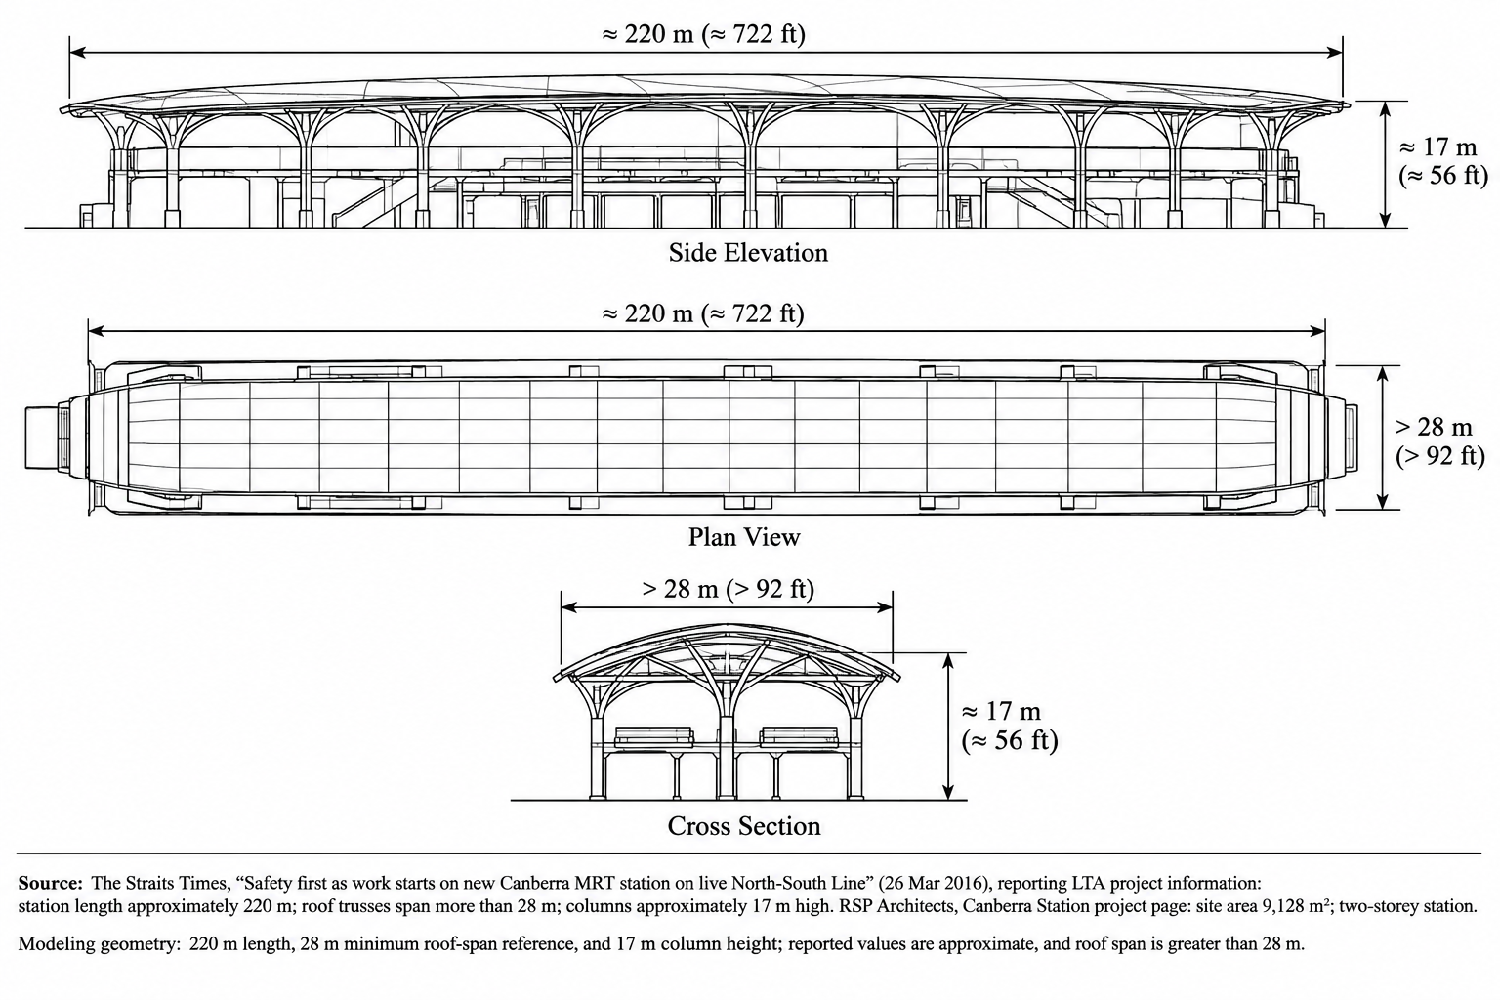
\includegraphics[width=0.96\linewidth]{figures/13_canberra_station.pdf}
\caption{User-supplied Canberra station schematic, retained as a separate PDF. Approximate structural dimensions are contextual references; the drawing is not an as-built survey or a map of the calculation zones. Sources identified in the drawing are listed in \cite{canberra-dimensions,canberra-rsp}.}
\label{fig:canberra}
\end{figure}

\noindent\textbf{Geometry and scope.} Figure~\ref{fig:canberra} labels approximately 220 m station length, roof-truss span over 28 m, and roughly 17 m columns. The column height is not platform-to-roof clearance; the roof span includes non-waiting space. Neither their product nor the site area specifies the occupied air volume. We instead define an explicit station-scale planning scenario. Taking the approximately 220 m length as a reference, assume an aggregate waiting-strip width $b=6$ m and usable fraction $\alpha=0.8$, giving
\begin{equation}
 A_{\mathrm{occ}}=\alpha Lb=1056\,\mathrm{m^2}.
\label{eq:canberra-area}
\end{equation}
Neither $b$ nor $\alpha$ is measured: they represent waiting space after excluding tracks, access obstructions and non-waiting portions. Three equal aggregate zones of $352\,\mathrm{m^2}$ represent access-side, sheltered-core and exposed-edge conditions. Their assumed effective mixing height is 4 m, giving $1408\,\mathrm{m^3}$ per zone. These are functional control volumes, not surveyed platform compartments. This formulation uses the station's scale without treating column height or site area as occupied volume.

\subsection{What changes from the bus model, and why}

The service objective is unchanged. The station roof and partial enclosure motivate air and surface storage, while recirculation can accumulate moisture. Passenger arrivals and boarding alter both heat loads and demand over time. We replace prescribed temperature/humidity fields with coupled zone balances. The site's greenery is not assigned an unsupported numerical cooling credit; its effect would enter measured surface temperatures and envelope parameters.

\begin{table}[!ht]
\centering\small
\caption{Revisions to the bus model and their purpose.}
\label{tab:rail-changes}
\begin{tabularx}{\linewidth}{@{}>{\raggedright\arraybackslash}p{0.25\linewidth}>{\raggedright\arraybackslash}X>{\raggedright\arraybackslash}X@{}}
\toprule
Revision & Why it is needed & Added capability\\
\midrule
Air and surface storage & Partial enclosure allows thermal memory. & Predict warm-up, lag and residual heat.\\
Dynamic moisture and zone exchange & Recirculation changes inlet humidity; openings connect different regions. & Calculate evaporative feedback and dilution.\\
Time-dependent passengers & Arrivals and boarding change both loads and service demand. & Count time-resolved person-hours and crowd heat/moisture.\\
Device counts and service coverage & Cooling demand and passenger density vary across a large station. & Select quantities and locations using total power and passenger service.\\
\bottomrule
\end{tabularx}
\end{table}

\subsection{Coupled heat, moisture, and surface balances}

Following the control-volume structure of building heat and moisture balances \cite{epzone}, let each zone store moist-air enthalpy $h_z$ (J/kg dry air), humidity ratio $w_z$ (kg/kg dry air), and an effective roof/wall inner-surface temperature $T_{m,z}$. The air is well mixed within each zone. Its dry-air mass is approximated as constant, $M_z=\rho_{da,o}V_z$, with outdoor reference density. This is a reduced model, not an EnergyPlus or CFD simulation.

Define the exchange operator, for either $x=h$ or $w$, as
\begin{equation}
 \mathcal L_z(x)=\dot m_{0z}(x_o-x_z)+\sum_{j\ne z}\dot m_{zj}(x_j-x_z),
 \qquad \dot m_{0z}=M_z\lambda_z/3600.
\label{eq:rail-exchange}
\end{equation}
Here $\lambda_z$ is the assumed outdoor air-change rate in h$^{-1}$. Each exchange represents equal entering and leaving dry-air flow; adjacent-zone rates satisfy $\dot m_{zj}=\dot m_{jz}$. Wind, buoyancy and opening geometry can affect outdoor exchange \cite{ventilation}; a prescribed train-cycle pulse tests that uncertainty without claiming a station-specific piston-flow law.

With $x_{zk}$ devices of type $k$ in zone $z$, unit recirculation $\dot m_k$ (kg dry air/s), and time in seconds, our balances are
\begin{align}
 M_z\dot h_z={}&\mathcal L_z(h)+H_{ma,z}(T_{m,z}-T_z)
 +n_zq_c+n_zg h_v(T_z)+P_z
 +\sum_k x_{zk}\dot m_k(h_{e,zk}-h_z),\label{eq:rail-enthalpy}\\
 M_z\dot w_z={}&\mathcal L_z(w)+n_zg+
 \sum_k x_{zk}\dot m_k(w_{e,zk}-w_z),\label{eq:rail-moisture}\\
 C_{m,z}\dot T_{m,z}={}&H_{mo,z}(T_o-T_{m,z})+Q_{\mathrm{sol},z}
 +n_zq_r-H_{ma,z}(T_{m,z}-T_z).\label{eq:rail-surface}
\end{align}
The per-person inputs are convective heat $q_c$, radiative heat $q_r$, and water-vapor generation $g$. Vapor enters with $h_v(T)=2501000+1860T$ J/kg; no additional latent-heat term is added. Total device power $P_z=1000\sum_k x_{zk}p_k$ (W), with unit powers $p_k$ in kW, is assumed to dissipate locally as sensible heat. Pump power is already included in the device total. Conductances $H$ have units W/K, surface capacity $C_m$ has units J/K, and $Q_{\mathrm{sol}}$ is an effective absorbed envelope load. The opposite signs of the air--surface term conserve internal energy.

Air temperature is recovered from $T_z=(h_z-2501000w_z)/(1006+1860w_z)$. A shaded longwave approximation for the surface contribution to comfort \cite{thermalcomfort} gives
\begin{equation}
 T_{r,z}=\left[F_z(T_{m,z}+273.15)^4+(1-F_z)(T_{r,o}+273.15)^4\right]^{1/4}-273.15.
\label{eq:rail-mrt}
\end{equation}
$F_z$ is an assumed effective view fraction; the example sets external radiant temperature $T_{r,o}=T_o$, while keeping it a separate input. Direct sun on passengers and detailed radiative asymmetry are excluded.

\noindent\textbf{Device mechanisms.} A adds air movement and electrical heat, with $\dot m_A=0$. B/C recirculate local air: at every step Eq.~\eqref{eq:outlet} is evaluated using the \emph{current zone inlet}, rather than fixed outdoor conditions. Their approximate outlet enthalpy remains $h_{e,zk}=h_z$, while $w_{e,zk}>w_z$ when evaporation occurs. Thus evaporation can lower dry-bulb temperature without removing moist-air enthalpy. Rising local moisture reduces subsequent wet-bulb depression. The earlier fixed mixing fractions are replaced by these explicit flow balances. Local passenger air speeds remain stated assumptions, rather than solutions of a momentum model.

\subsection{Equipment selection, allocation, and coverage}

Let $x_{zk}\in\mathbb Z_{\ge0}$ be the number of devices of type $k\in\{A,B,C\}$ in zone $z$. A $3\times3$ count matrix specifies a candidate installation, allowing quantities and device types to vary by zone. Each candidate is evaluated through the resulting shared thermal environment: all operating units contribute heat and electricity, and evaporative units also contribute moisture.

We use assumed, non-overlapping service footprints $a_A=20$, $a_B=30$ and $a_C=40\,\mathrm{m^2}$ per unit. These are comparison inputs, not manufacturer coverage ratings. For uniform passenger density within a zone, define
\begin{equation}
 f_{zk}=\frac{x_{zk}a_k}{A_z},\qquad
 f_{z0}=1-\sum_k f_{zk}\ge0,\qquad \sum_kx_{zk}a_k\le A_z.
\label{eq:coverage}
\end{equation}
The uncovered fraction experiences local speed $v_0$; each covered subgroup experiences its device-specific speed $v_{zk}$. We average \emph{discomfort}, not velocities or device efficiencies:
\begin{equation}
 \overline D_{s,z}(t)=f_{z0}D[\Theta(T_z,T_{r,z},v_0,\phi_z)]
 +\sum_k f_{zk}D[\Theta(T_z,T_{r,z},v_{zk},\phi_z)].
\label{eq:mixed-discomfort}
\end{equation}
All subgroups share the zone's mixed temperature, humidity and radiant environment; an uncovered passenger can therefore still experience indirect cooling or humidification. The coverage fraction measures direct air-movement service, not a boundary of all thermal influence. The formulation represents distributed equipment with separate service footprints. Co-located jets, overlapping footprints and series arrangements require a resolved airflow model.

\subsection{Canberra scenario and comparable deployment tests}

We assume $33\,^{\circ}\mathrm C$ and $70\%$ outdoor RH for a hot, humid Canberra scenario. Singapore's weather service describes typical daytime maxima of $31$--$33\,^{\circ}\mathrm C$ and high humidity, with rain-free afternoon RH around $60\%$ \cite{singapore-climate}. Our pair is a scenario, not a simultaneous observation at the station. SET retains $1.2$ met, $0.5$ clo, and the common $26\,^{\circ}\mathrm C$ reference.

\begin{table}[!ht]
\centering\small
\caption{Station-scale scenario inputs: all numerical operating parameters below are assumptions.}
\label{tab:rail-inputs}
\begin{tabularx}{\linewidth}{@{}>{\raggedright\arraybackslash}p{0.27\linewidth}>{\raggedright\arraybackslash}X@{}}
\toprule
Input & Assumed value and interpretation\\
\midrule
People and train cycle & An assumed 15-min stress-test cycle, not the actual timetable. Zone counts rise from $(26.4,44,17.6)$ to $(88,198,66)$, then reset; fractional values represent mean counts.\\
Outdoor and zone exchange & Base ACH $(8,4,10)$ h$^{-1}$, plus $(8,4,12)$ in the last 2 min; adjacent-zone exchange $0.88$ kg dry air/s.\\
Surface response, per zone & $C_m=17.6$ MJ/K; $H_{ma}=880$, $H_{mo}=1760$ W/K; absorbed load $3520$ W; view fractions $(0.55,0.85,0.55)$.\\
Human sources & Convection $45$ W, radiation $30$ W, vapor $45/(2.45\times10^6)$ kg/s per person.\\
Device powers and flows & $p_{A/B/C}=0.25/1.2/2.5$ kW per unit; B/C recirculate $0.60/1.20$ kg dry air/s per unit, with $\varepsilon=0.70$ and $5/8\,^{\circ}\mathrm C$ outlet-drop caps.\\
Speeds at covered locations & A $(0.60,1.00,0.50)$, B $(0.50,0.80,0.45)$, C $(0.75,1.00,0.60)$ m/s; uncovered locations $0.20$ m/s.\\
\bottomrule
\end{tabularx}
\end{table}

The same occupied area, thermal properties, load densities and passenger schedule are used for every candidate. This holds demand constant while equipment quantities and allocation change. The architectural sources establish the venue context; the assumed operating conditions and coverage parameters define the numerical comparison.

We first compare six benchmark configurations at the same direct-service footprint: $240\,\mathrm{m^2}$ per zone, or $68.2\%$ of the assumed occupied area. Per-zone counts $(x_A,x_B,x_C)$ are $(12,0,0)$, $(0,8,0)$, $(0,0,6)$, $(6,4,0)$, $(6,0,3)$ and $(3,2,3)$. Whole-station totals are respectively 36, 24, 18, 30, 27 and 24 units. Device-count sweeps then quantify the energy needed for wider coverage, and a fixed-inventory redistribution test isolates the effect of allocation. Together these comparisons address type, quantity and placement.

The scenario first receives a prescribed two-hour uncooled warm-up from outdoor air and surface conditions. All strategies then start from that \emph{same} warm-up state and are assessed for two hours. The independent no-device trajectory uses identical passengers, weather and exchange. All candidates operate for the full assessment; the denominator measures incremental cooling-device electricity, not the whole station electricity bill. This specifies a common prior history; it is not a claim that a periodic steady state has been reached. It prevents stored cooling from being supplied free at the initial time. Later benefits beyond the assessment horizon are not credited.

\subsection{Comparing service, coverage, and electricity}

Retain signed relief against the matched baseline, now using the coverage-weighted discomfort:
\begin{equation}
 U_s=\int_0^{2\mathrm h}\sum_z n_z(t)[D_{0,z}(t)-\overline D_{s,z}(t)]\,dt,
 \qquad E_s=\int_0^{2\mathrm h}\sum_{z,k}x_{zk}p_k\,dt,
 \qquad \eta_s=U_s/E_s.
\label{eq:rail-efficiency}
\end{equation}
The units remain person$\cdot{}^{\circ}\mathrm C\cdot$h/kWh. Report mean remaining discomfort $\overline R_s=\int\sum_z n_z\overline D_{s,z}\,dt/\int\sum_z n_z\,dt$ alongside $\eta_s$ and coverage. Selection proceeds in two steps: retain candidates that meet the specified remaining-discomfort and person-hour coverage requirements, then choose the lowest-energy candidate. Because acceptance thresholds have not been specified for this scenario, we report the energy--discomfort frontier and coverage of the tested candidates. This identifies the available choices while leaving the final device count dependent on service requirements.

The two-hour evaluation contains $440$ person-hours; the no-device mean remaining SET excess is $10.57\,^{\circ}\mathrm C$. At equal $68.2\%$ coverage, A36 is the preferred benchmark: its 36 fans use 18.0 kWh and leave $9.06\,^{\circ}\mathrm C$, giving both the lowest electricity use and the lowest remaining discomfort among the six configurations. B24 and C18 use 57.6 and 90.0 kWh and leave $9.45$ and $9.42\,^{\circ}\mathrm C$; AB30, AC27 and ABC24 use 37.8, 54.0 and 63.9 kWh and leave $9.18$, $9.15$ and $9.28\,^{\circ}\mathrm C$. The modeled advantage comes from air movement at low electrical input, while evaporative devices add humidity and consume more power. Across all 24 candidates, the sampled energy--discomfort frontier consists of fan configurations with different counts. Selecting a count therefore depends on the required coverage and relief, rather than the efficiency ratio alone.

\noindent\textbf{Allocating a fixed equipment inventory.} AB30 places $(6,4,0)$ units in each zone. Redistributing the same 18 A and 12 B units as $(3,4,0)$, $(12,3,0)$ and $(3,5,0)$ gives AB30-R. Both consume 37.8 kWh and cover $68.2\%$ of area, but the person-hour coverage $\int\sum_z n_z(1-f_{z0})dt/\int\sum_z n_zdt$ rises from $68.2\%$ to $76.2\%$. Mean remaining excess falls from $9.18$ to $8.92\,^{\circ}\mathrm C$, and efficiency rises from $16.12$ to $19.19$. The comparison shows that directing equipment toward higher passenger demand can improve service without adding units or electricity. It tests allocation for a fixed inventory; the overall choice follows the same energy and service criteria used for every candidate.

\noindent\textbf{Coverage uncertainty.} Multiplying all footprints by $0.75$, $1$ and $1.25$ changes benchmark direct coverage to $51.1\%$, $68.2\%$ and $85.2\%$. A36's mean remaining excess changes from $9.49$ to $9.06$ to $8.63\,^{\circ}\mathrm C$ without changing electricity. A36 retains the lowest energy use and remaining discomfort among the six benchmarks at each common multiplier; the B/C and AB/AC rankings change. This tests a common coverage error, not independent errors in each device type; measured throw and passenger locations remain important. High remaining discomfort also shows that relative efficiency alone does not establish adequate service.

\begin{figure}[!ht]
\centering
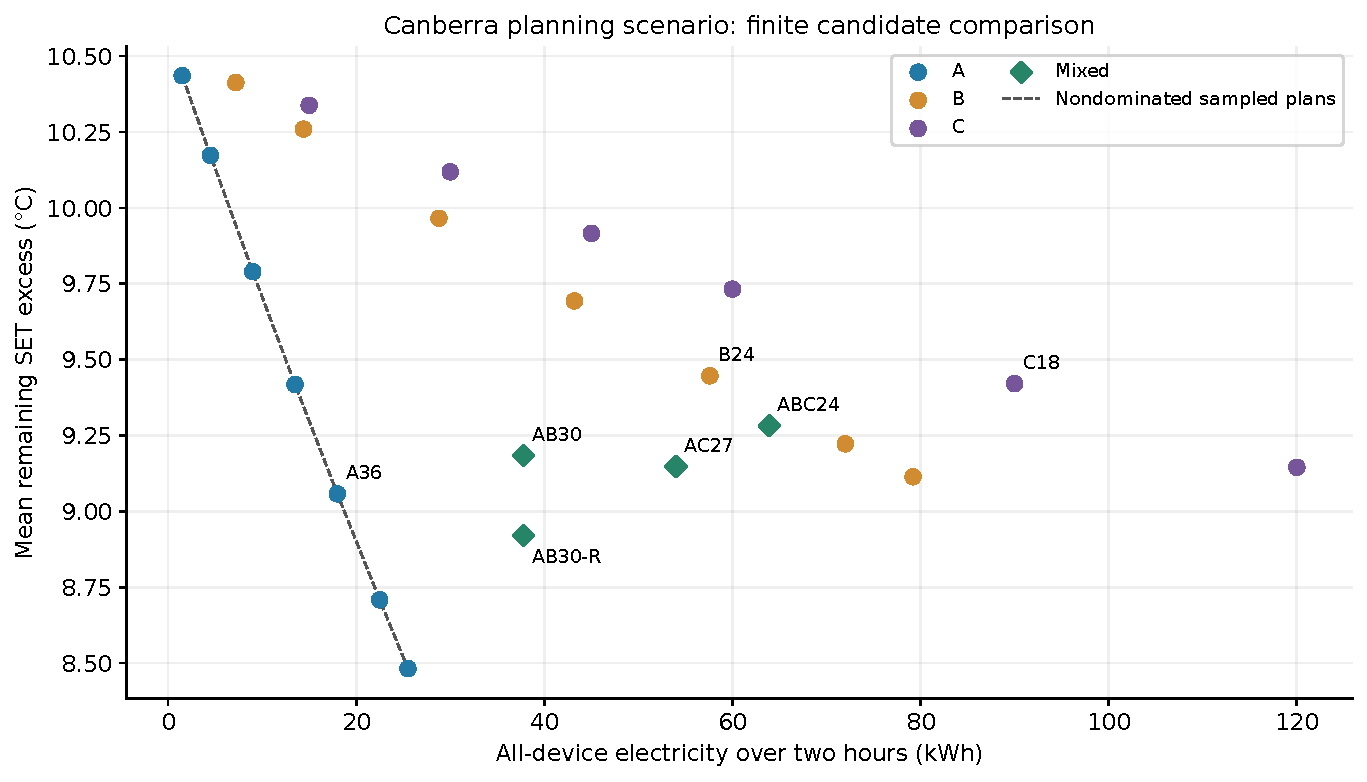
\includegraphics[width=0.90\linewidth]{figures/14_deployment_tradeoff.pdf}
\caption{Energy--discomfort tradeoffs for 24 candidate configurations. The dashed line marks the nondominated candidates; required passenger coverage guides selection.}
\label{fig:deployment-tradeoff}
\end{figure}

\begin{figure}[!ht]
\centering
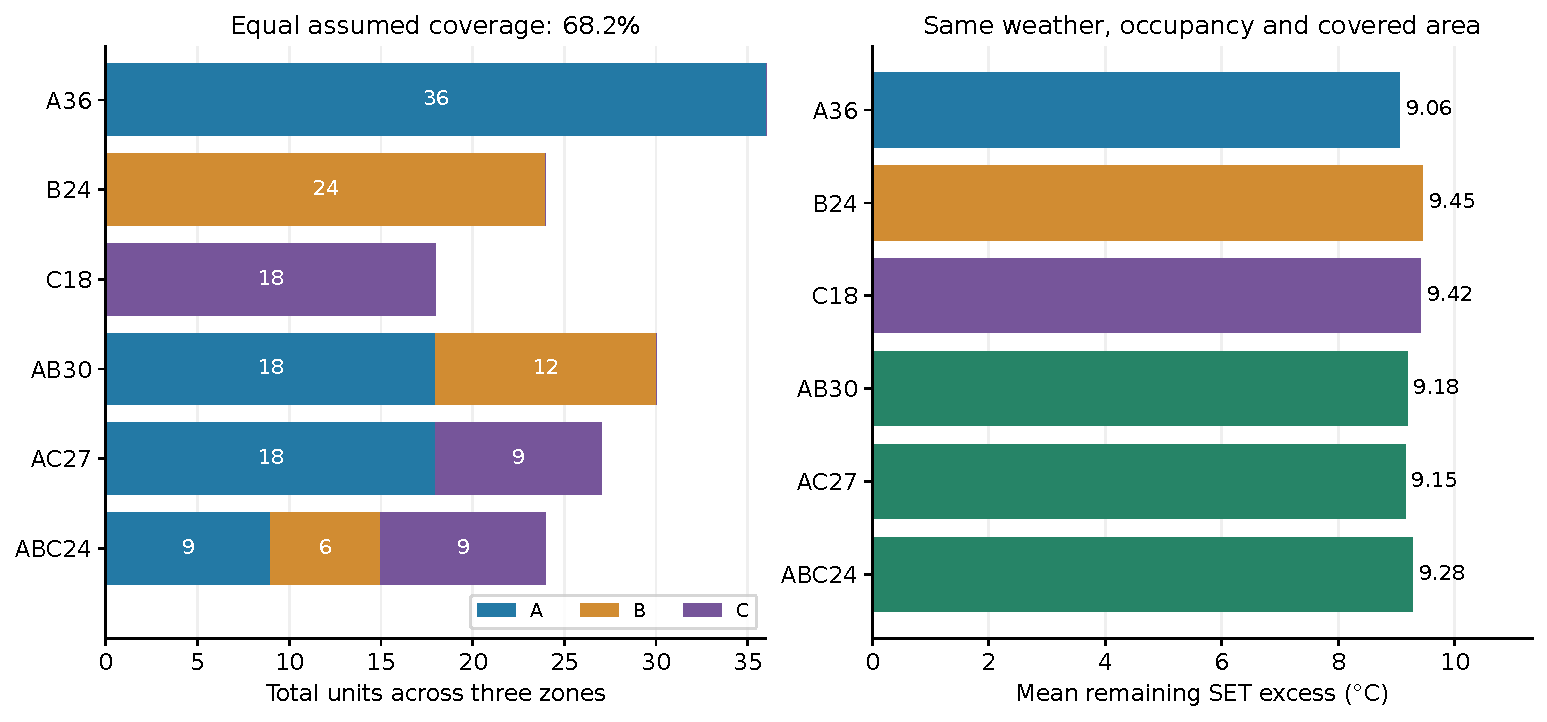
\includegraphics[width=0.90\linewidth]{figures/15_deployment_mix.pdf}
\caption{Equal-footprint deployment comparison: counts and performance at $68.2\%$ direct-service coverage. All devices contribute to the shared heat/moisture balances and total electricity.}
\label{fig:deployment-mix}
\end{figure}

\begin{figure}[!ht]
\centering
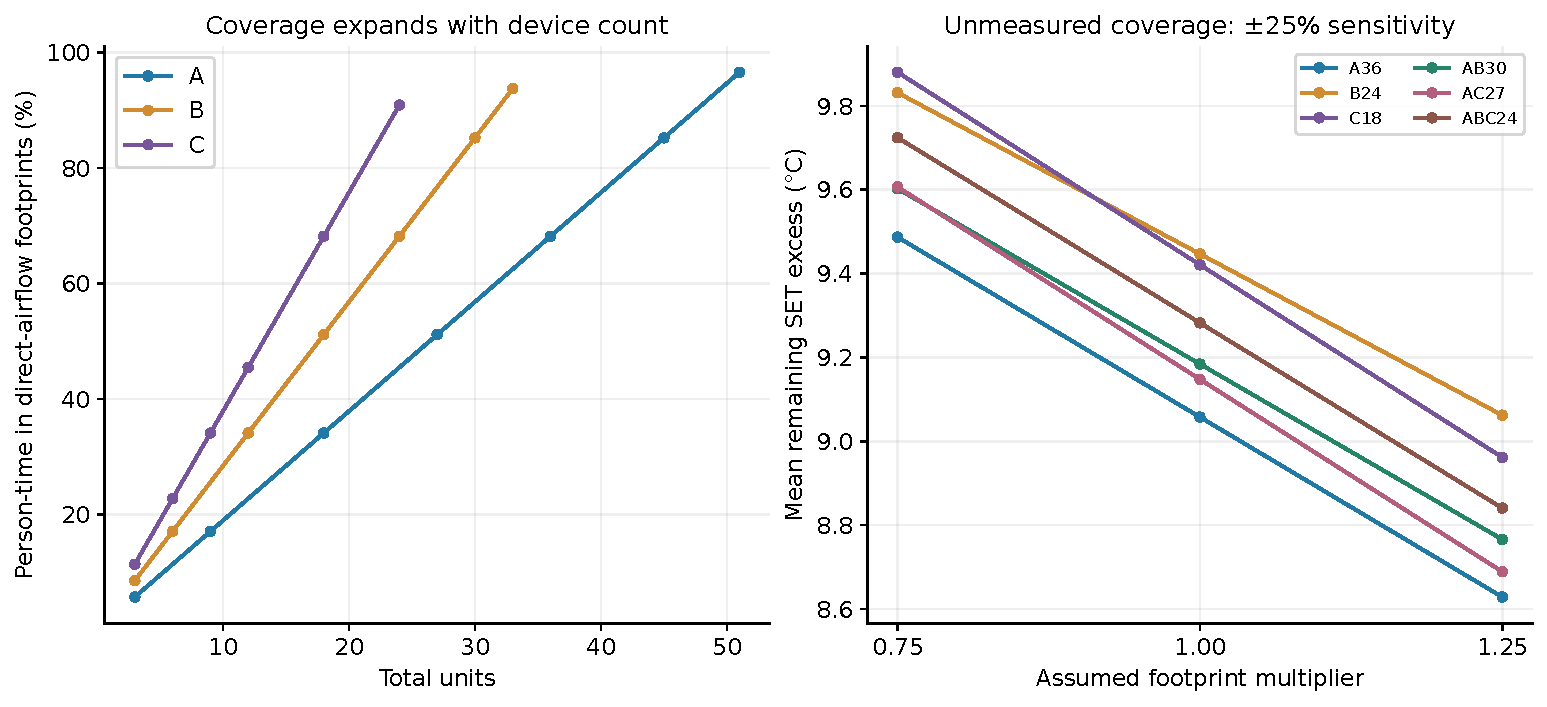
\includegraphics[width=\linewidth]{figures/16_deployment_coverage.pdf}
\caption{Device-count and assumed-footprint sensitivity. Changing footprint affects direct-service fractions; numerical coverage is not a verified equipment rating.}
\label{fig:deployment-coverage}
\end{figure}

\subsection{Usefulness, station-wide transfer, and verification}

By resolving thermal storage, moisture accumulation and changing passenger loads, the revised model links equipment selection to conditions throughout the waiting period.

\noindent\begin{minipage}{\linewidth}
\noindent\textbf{Limits of the planning scale.} The selection results depend on effective platform area, air exchange, device throw and passenger distribution. Field measurements and layout constraints, including electrical capacity, stairs and benches, are needed to specify an installation. Shared zone temperatures and separate service footprints approximate equipment delivery; they do not resolve extra cooling in an evaporative outlet jet. The reported ranking therefore applies to the stated scenario and should be reassessed when these inputs are calibrated.
\end{minipage}

\Needspace{7\baselineskip}
\noindent\textbf{Verification.} RK4 uses a 20 s step aligned with schedule boundaries. Repeating the three mixed benchmarks at 10 s changes efficiency by less than $0.001\%$ and mean remaining SET excess by less than $10^{-5}\,^{\circ}\mathrm C$. Eleven checks cover integer counts, non-overlapping coverage, full electricity, heat/moisture conservation, $U_s+R_s=R_0$, valid psychrometrics and SET, reduction to a pure-device model, zero-occupancy accounting, signed adverse effects, coverage weights and convergence. Maximum candidate energy and vapor residuals are below $4\times10^{-6}$ J and $2\times10^{-13}$ kg. These verify implementation consistency, not field accuracy.

The accompanying \texttt{deployment\_model} folder contains the scenario, solver, CSV trajectories, initial states, sensitivity results and verification records. SET remains a quasi-steady human-response calculation even though the environment is dynamic. The model neglects surface moisture sorption, condensation, detailed stratification and direct solar exposure. It stops on invalid humidity or SET inputs instead of hiding them. Outdoor exchange, effective occupied area and coverage need field calibration before operational recommendations.
